% ------------------------------------------------------------------------------
% TYPO3 CMS 7.4 - What's New (English Version)
%
% @author	Michael Schams <schams.net>
% @license	Creative Commons BY-NC-SA 3.0
% @link		http://typo3.org/download/release-notes/whats-new/
% @language	English
% ------------------------------------------------------------------------------
% LTXE-CHAPTER-UID:		0dbe76ce-5948c314-454b95fd-543cb62c
% LTXE-CHAPTER-NAME:	Backend User Interface
% ------------------------------------------------------------------------------

\section{Backend User Interface}
\begin{frame}[fragile]
	\frametitle{Backend User Interface}

	\begin{center}\huge{Chapter 1:}\end{center}
	\begin{center}\huge{\color{typo3darkgrey}\textbf{Backend User Interface}}\end{center}

\end{frame}

% ------------------------------------------------------------------------------
% LTXE-SLIDE-START
% LTXE-SLIDE-UID:		464d4ba6-dab07499-0cd5f168-552e9729
% LTXE-SLIDE-ORIGIN:	8080f469-3c5592f0-dc25ad87-894c2648 German
% LTXE-SLIDE-TITLE:		Feature: #48947 - Avatars for backend users
% LTXE-SLIDE-REFERENCE:	Feature-48947-AvatarsForBackendUsers.rst
% ------------------------------------------------------------------------------
\begin{frame}[fragile]
	\frametitle{Backend User Interface}
	\framesubtitle{Avatars for Backend Users}

	To improve the user experience in collaborative content editing, backend users can use avatars now.
	These small user images are shown in the topbar, users list and other places.

	\begin{figure}
		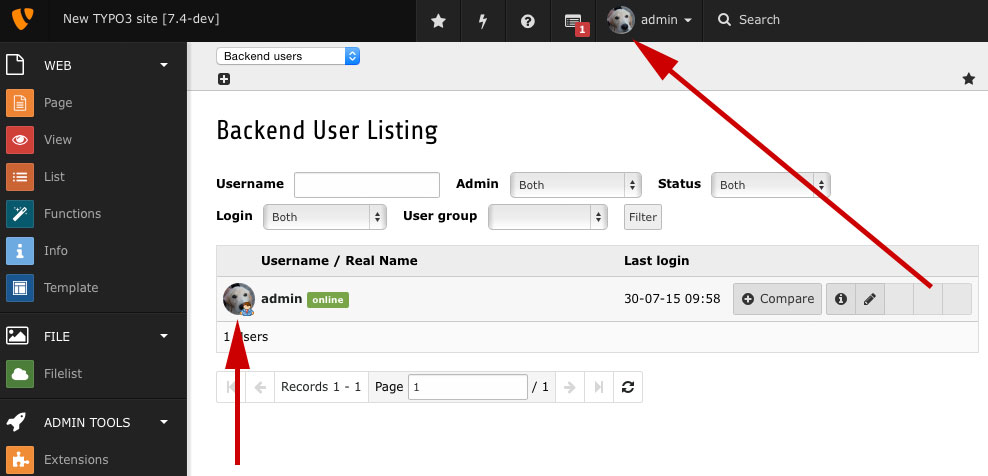
\includegraphics[width=0.9\linewidth]{BackendUserInterface/48947.jpg}
	\end{figure}

\end{frame}

% ------------------------------------------------------------------------------
% LTXE-SLIDE-START
% LTXE-SLIDE-UID:		89f348c8-db045eff-5dfc4f42-da1a2cfa
% LTXE-SLIDE-ORIGIN:	b0f7e15a-7cc72aaa-79738ec7-643c5cec German
% LTXE-SLIDE-TITLE:		Feature: #56133 - Replace file feature for fal file list
% LTXE-SLIDE-REFERENCE:	Feature-56133-ReplaceFileFeatureForFalFileList.rst
% ------------------------------------------------------------------------------
\begin{frame}[fragile]
	\frametitle{Backend User Interface}
	\framesubtitle{Replace Files}

	Files in the FAL record list can now be \textbf{replaced} (requires enabled "extended view").
	Filename of the existing file can be retained or updated.

	\begin{figure}
		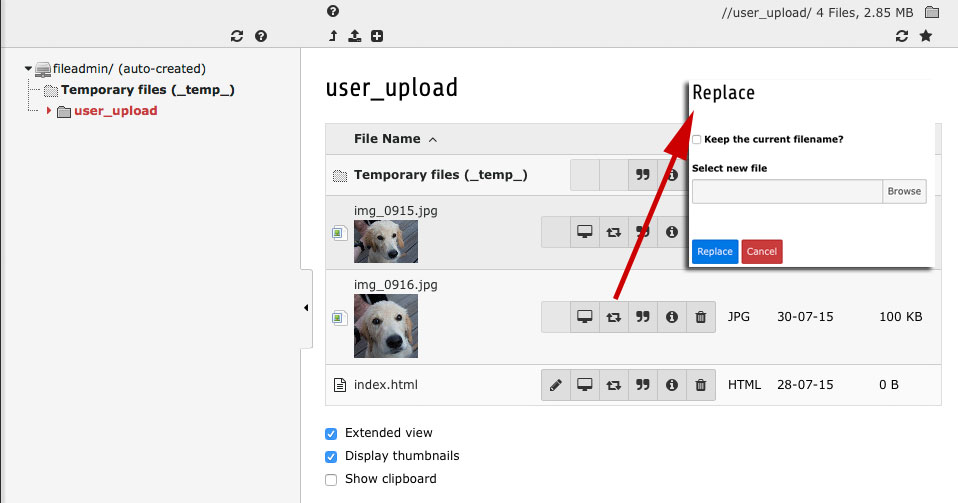
\includegraphics[width=0.75\linewidth]{BackendUserInterface/56133.jpg}
	\end{figure}

\end{frame}

% ------------------------------------------------------------------------------
% LTXE-SLIDE-START
% LTXE-SLIDE-UID:		7e5987f7-9a91ea61-8564c721-0f8d5e4a
% LTXE-SLIDE-ORIGIN:	613354cc-9475feef-bec620c5-31170549 German
% LTXE-SLIDE-TITLE:		Feature: #67574 - Display online status in backend user list
% LTXE-SLIDE-REFERENCE:	Feature-67574-DisplayOnlineStatusInBackendUserList.rst
% ------------------------------------------------------------------------------
\begin{frame}[fragile]
	\frametitle{Backend User Interface}
	\framesubtitle{Online Status of Backend Users}

	The online status of backend users is shown in module "Backend Users".

	\begin{figure}
		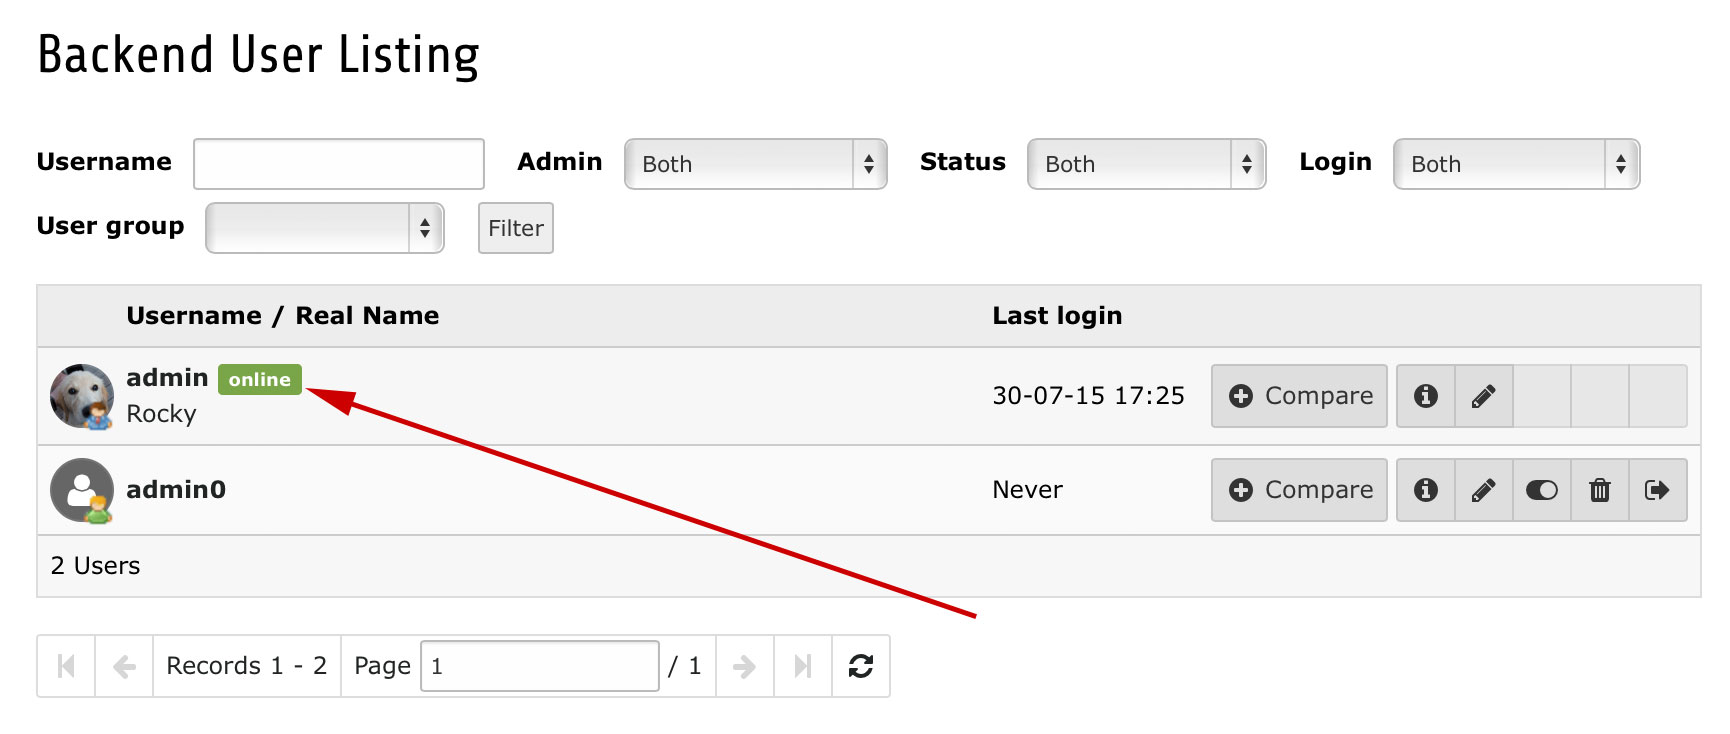
\includegraphics[width=0.9\linewidth]{BackendUserInterface/67574.jpg}
	\end{figure}

\end{frame}

% ------------------------------------------------------------------------------
% LTXE-SLIDE-START
% LTXE-SLIDE-UID:		0154fc51-74683590-ebbe8559-ce6a0d57
% LTXE-SLIDE-ORIGIN:	00c93fe2-9d128591-20b71814-13556f43 German
% LTXE-SLIDE-TITLE:		FormEngine: Drop "Show secondary options"
% LTXE-SLIDE-REFERENCE:	https://forge.typo3.org/issues/67753
% ------------------------------------------------------------------------------
\begin{frame}[fragile]
	\frametitle{Backend User Interface}
	\framesubtitle{Secondary Options Removed}

	The checkbox "Show secondary options (palettes)", the page TSconfig option \texttt{options.enableShowPalettes}
	and the TCA setting have been removed. The palettes are always visible and can not be hidden anymore.

	\begin{figure}
		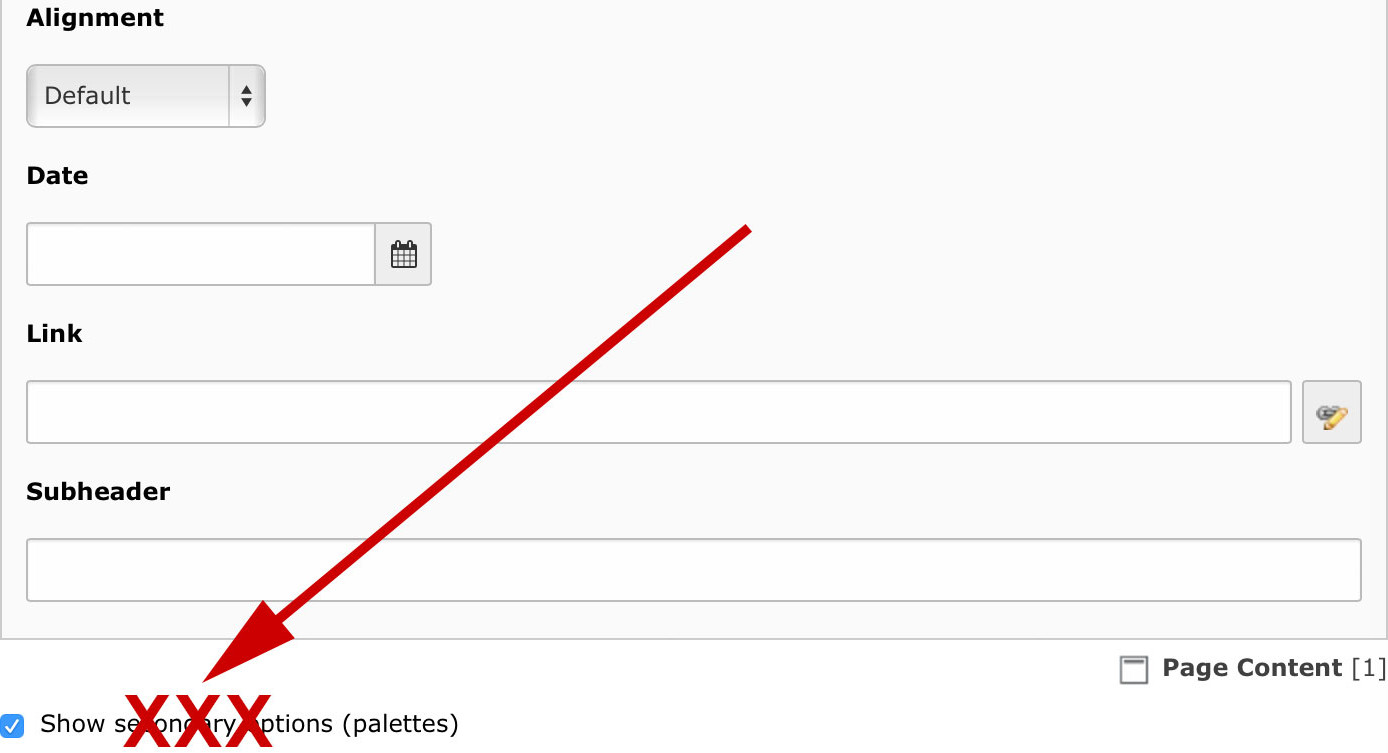
\includegraphics[width=0.7\linewidth]{BackendUserInterface/67753.jpg}
	\end{figure}

\end{frame}

% ------------------------------------------------------------------------------
% LTXE-SLIDE-START
% LTXE-SLIDE-UID:		f9b24e36-28e8872c-41297de9-52467554
% LTXE-SLIDE-ORIGIN:	bab4e93d-0a6d4612-41b2f67e-47c37ff7 German
% LTXE-SLIDE-TITLE:		Feature: #67578 - Add description-field for backend-users
% LTXE-SLIDE-REFERENCE:	Feature-67578-AddDescriptionFieldForBeUsers.rst
% ------------------------------------------------------------------------------
\begin{frame}[fragile]
	\frametitle{Backend User Interface}
	\framesubtitle{Description for Backend Users}

	A new field "Description" has been added to backend user records.

	\begin{figure}
		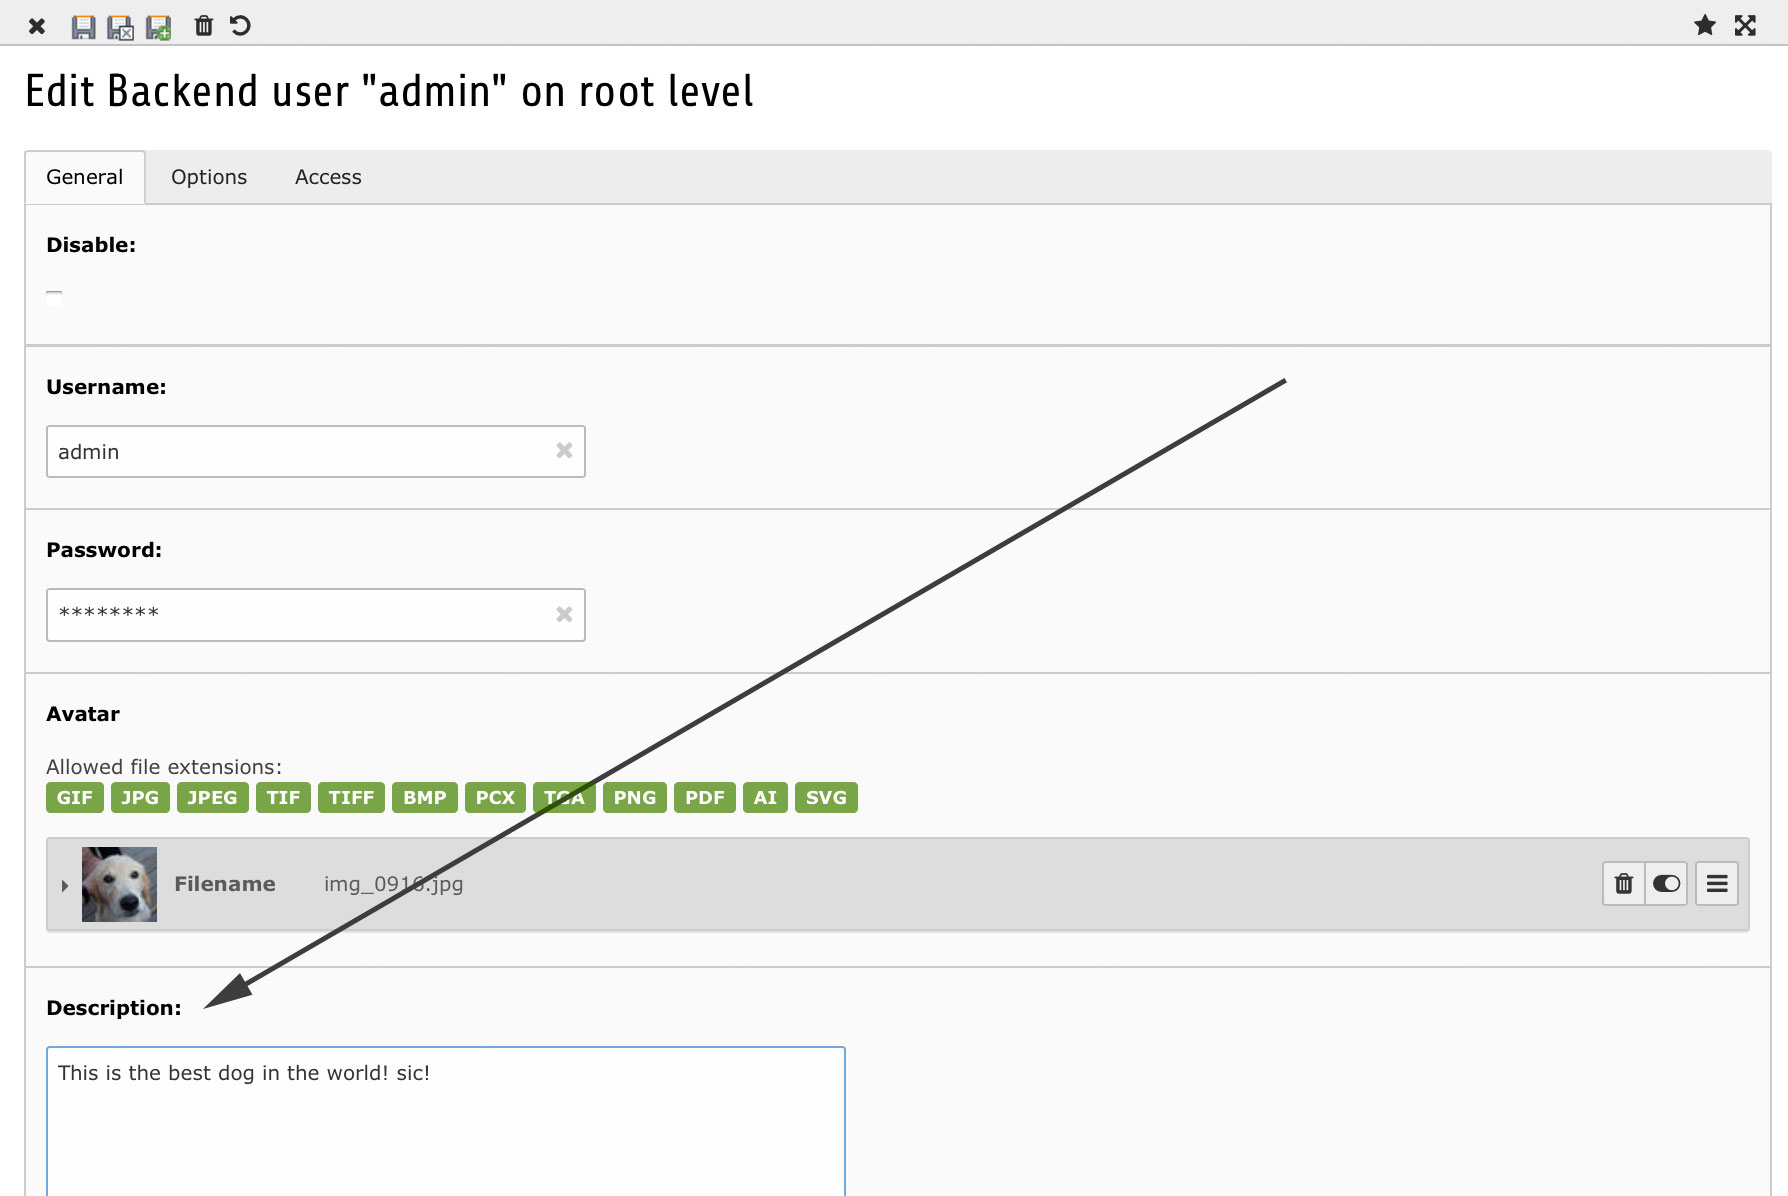
\includegraphics[width=0.7\linewidth]{BackendUserInterface/67578.jpg}
	\end{figure}

\end{frame}

% ------------------------------------------------------------------------------
% LTXE-SLIDE-START
% LTXE-SLIDE-UID:		83db5442-fa2edfcc-925dd5b6-4afe26f5
% LTXE-SLIDE-ORIGIN:	649bd9ee-240381c8-950424ea-f032775b German
% LTXE-SLIDE-TITLE:		Feature: #67603 - Introduce TCA > ctrl > descriptionColumn
% LTXE-SLIDE-REFERENCE:	Feature-67603-IntroduceTcaDescriptionColumn.rst
% ------------------------------------------------------------------------------
\begin{frame}[fragile]
	\frametitle{Backend User Interface}
	\framesubtitle{Description for Table Columns}

	By configuring a column (usually \texttt{description}) in TCA setting \texttt{['TCA']['ctrl']['descriptionColumn']},
	a description can be shown (improves usability for editors and administrators).

	\begin{figure}
		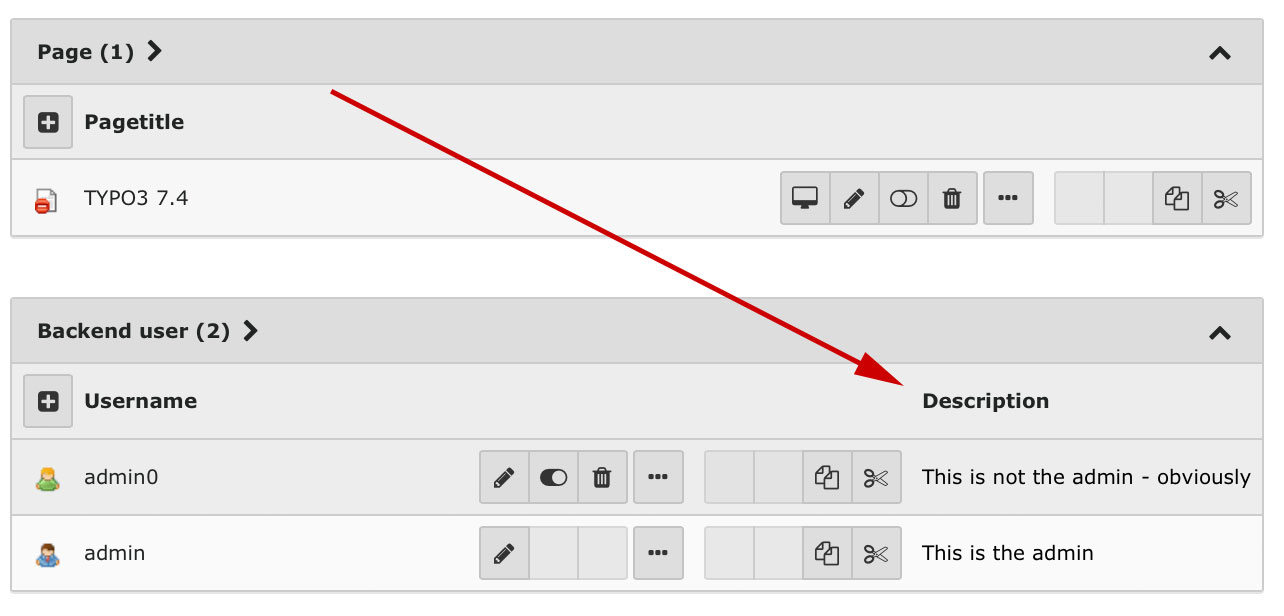
\includegraphics[width=0.7\linewidth]{BackendUserInterface/67603.jpg}
	\end{figure}

\end{frame}

% ------------------------------------------------------------------------------
% LTXE-SLIDE-START
% LTXE-SLIDE-UID:		7c5400a9-c4b667f3-1a0c046a-9dd3b6a9
% LTXE-SLIDE-ORIGIN:	2eeaec46-1929743b-8e6f9285-13d20d3c German
% LTXE-SLIDE-TITLE:		Feature: #59570 - Add description-field for filemounts
% LTXE-SLIDE-REFERENCE:	Feature-59570-AddDescriptionFieldForFilemounts.rst
% ------------------------------------------------------------------------------
\begin{frame}[fragile]
	\frametitle{Backend User Interface}
	\framesubtitle{Description for Filemounts}

	A new field "Description" has been added to filemount records.
	The field allows administrators to add a short description what a certain filemount should be used for,
	which documents it may contain, etc.

	\begin{figure}
		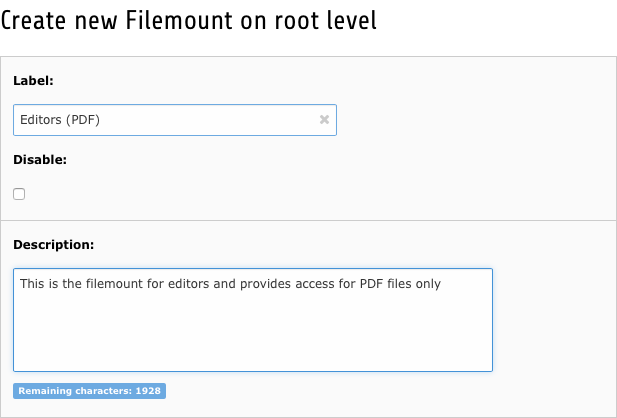
\includegraphics[width=0.55\linewidth]{BackendUserInterface/59570.png}
	\end{figure}

\end{frame}

% ------------------------------------------------------------------------------
% LTXE-SLIDE-START
% LTXE-SLIDE-UID:		d00f63c4-05272792-21a0a301-4d6a726c
% LTXE-SLIDE-ORIGIN:	879b1dda-9167d830-373f7457-0391ebee German
% LTXE-SLIDE-TITLE:		Feature: #68197 - Show a dialog for existing files on upload
% LTXE-SLIDE-REFERENCE:	Feature-68197-ShowADialogForExistingFilesOnUpload.rst
% ------------------------------------------------------------------------------
\begin{frame}[fragile]
	\frametitle{Backend User Interface}
	\framesubtitle{Dialog for Existing Files on Upload}

	If a file upload would overwrite an existing file, a dialog is shown, asking the user
	to choose an action (e.g. replace, rename or skip).

	\begin{figure}
		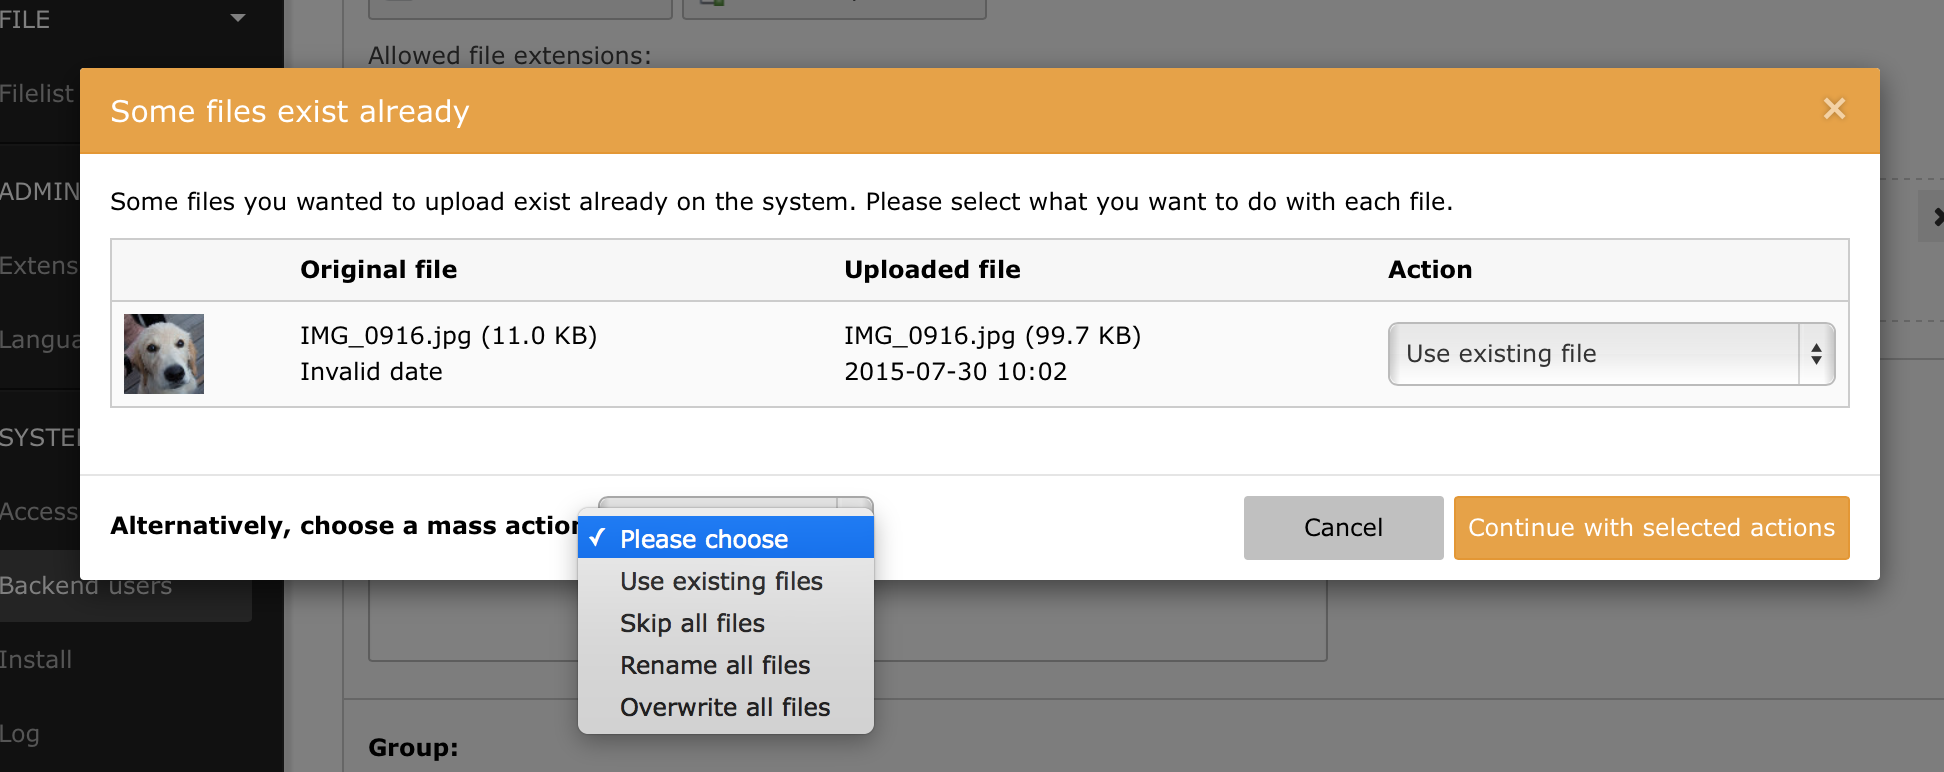
\includegraphics[width=0.9\linewidth]{BackendUserInterface/68197.png}
	\end{figure}

\end{frame}


% ------------------------------------------------------------------------------
% LTXE-SLIDE-START
% LTXE-SLIDE-UID:		31d7dd8e-a3c71be4-309850ab-45a7db72
% LTXE-SLIDE-ORIGIN:	f4baa7b8-2237ad1d-5c4be365-a845f207 German
% LTXE-SLIDE-TITLE:		Feature: #68218 - Lock edit for tt_content
% LTXE-SLIDE-REFERENCE:	Feature-68218-LockEditForTt_content.rst
% ------------------------------------------------------------------------------
\begin{frame}[fragile]
	\frametitle{Backend User Interface}
	\framesubtitle{Editing Content Elements Restriction}

	Content elements can now be restricted to be editable by admins only
	(similar to function "Restrict editing by non-Admins" for pages).

	\begin{figure}
		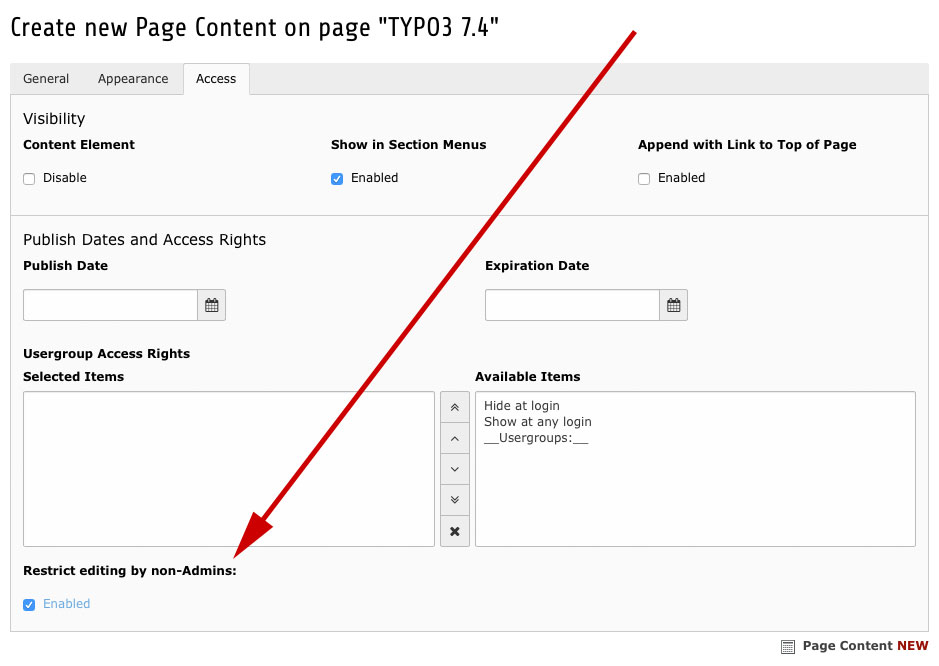
\includegraphics[width=0.6\linewidth]{BackendUserInterface/68218.jpg}
	\end{figure}

\end{frame}

% ------------------------------------------------------------------------------
% LTXE-SLIDE-START
% LTXE-SLIDE-UID:		4e60055a-266e3e24-7baa1613-1226575e
% LTXE-SLIDE-ORIGIN:	bc83e40f-9b7bac03-ea5f07c4-be27eb56 German
% LTXE-SLIDE-TITLE:		Feature: #68315 - Include pageTSconfig file (1)
% LTXE-SLIDE-REFERENCE:	Feature-68315-IncludeAPageTSconfigFileInPagePropertiesLikeTSStaticTemplates.rst
% ------------------------------------------------------------------------------
\begin{frame}[fragile]
	\frametitle{Backend User Interface}
	\framesubtitle{Include Static TSconfig Files (1)}

	In page properties an option allows to include a page TSconfig file
	(the same way as TypoScript static templates are included).

	\begin{figure}
		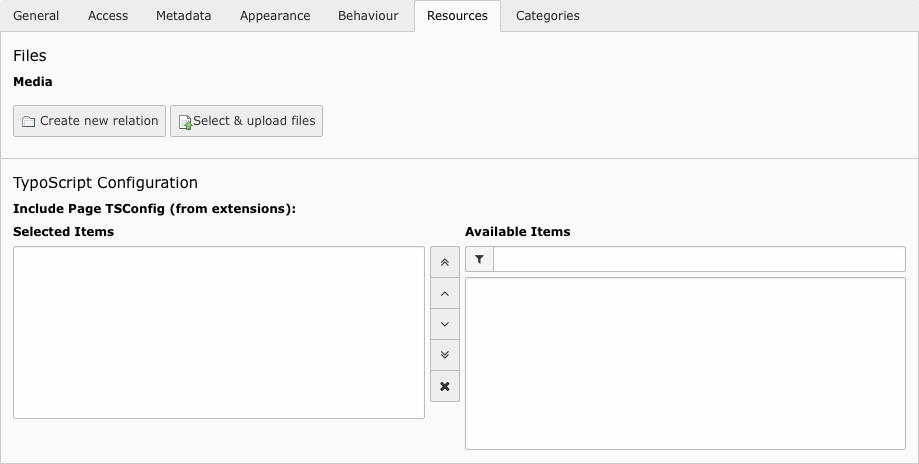
\includegraphics[width=0.8\linewidth]{BackendUserInterface/68315.png}
	\end{figure}

\end{frame}

% ------------------------------------------------------------------------------
% LTXE-SLIDE-START
% LTXE-SLIDE-UID:		4f5cb411-3ea84dfd-84edb16d-433b9fc5
% LTXE-SLIDE-ORIGIN:	9b7bac03-ea5f07c4-be27eb56-ac03e27e German
% LTXE-SLIDE-TITLE:		Feature: #68315 - Include pageTSconfig file (2)
% LTXE-SLIDE-REFERENCE:	Feature-68315-IncludeAPageTSconfigFileInPagePropertiesLikeTSStaticTemplates.rst
% ------------------------------------------------------------------------------
\begin{frame}[fragile]
	\frametitle{Backend User Interface}
	\framesubtitle{Include Static TSconfig Files (2)}

	% decrease font size for code listing
	\lstset{basicstyle=\tiny\ttfamily}

	The following method registers a page TSconfig file:

	\begin{lstlisting}
		\TYPO3\CMS\Core\Utility\ExtensionManagementUtility::registerPageTSConfigFile(
		  'extension_name',
		  'Configuration/PageTS/myPageTSconfigFile.txt',
		  'My special configuration'
		);
	\end{lstlisting}

\end{frame}

% ------------------------------------------------------------------------------
% LTXE-SLIDE-START
% LTXE-SLIDE-UID:		c00b2bfd-2c1b02b0-a7ef9cd0-62f147d2
% LTXE-SLIDE-ORIGIN:	f8d888b1-b93dcf4a-e20b976e-9a5c277e German
% LTXE-SLIDE-TITLE:		Feature: #68395 - Allow real copies of content elements into foreign languages
% LTXE-SLIDE-REFERENCE:	Feature-68395-AllowRealCopiesOfContentElementsIntoForeignLanguages.rst
% ------------------------------------------------------------------------------
\begin{frame}[fragile]
	\frametitle{Backend User Interface}
	\framesubtitle{Real Copies of Content Elements}

	A new button has been added to each column in the "Page" module which allows \textit{real} copies of content element
	into a language (not only references).

	\begin{figure}
		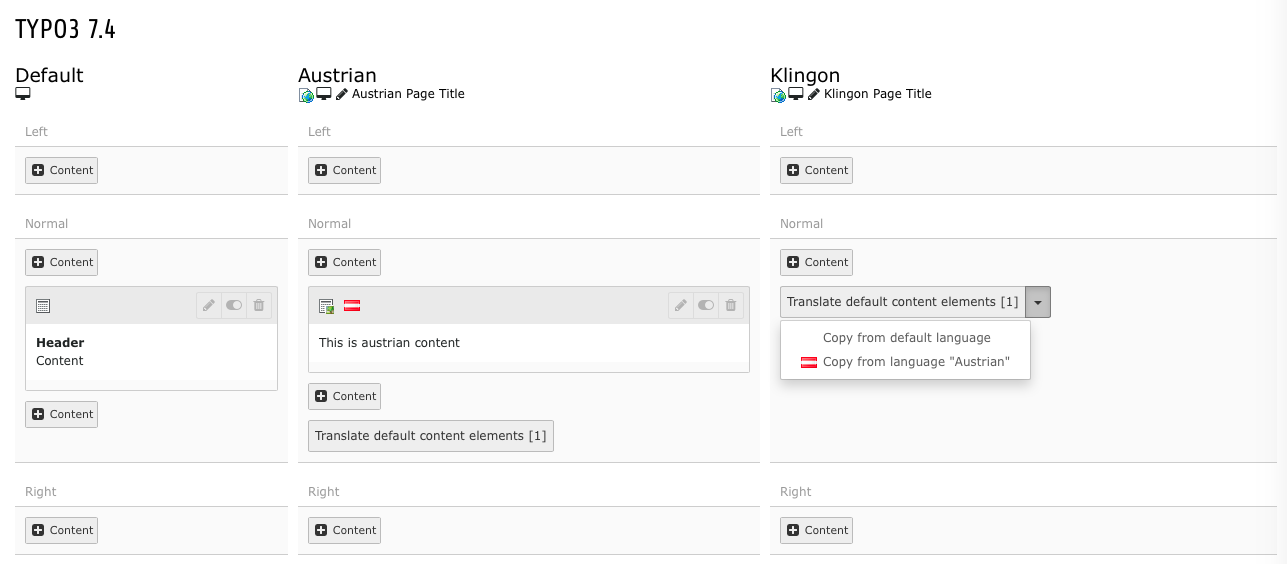
\includegraphics[width=0.9\linewidth]{BackendUserInterface/68395.png}
	\end{figure}

\end{frame}


